\documentclass[12pt]{article}
\usepackage{times}
\usepackage[english]{babel}
\usepackage[utf8x]{inputenc}
\usepackage[colorinlistoftodos]{todonotes}
\usepackage[margin=1in]{geometry}
\usepackage{graphicx}
\usepackage{epstopdf}
\usepackage{cite}
\usepackage{listings}
\usepackage{dtklogos}
\usepackage{wrapfig}
\usepackage{subfigure}
\usepackage{amsmath}
\usepackage{amsthm}
\usepackage{amssymb}
\usepackage{amscd}
\usepackage{caption}
\usepackage{etoolbox}
\usepackage{fancyhdr}
\usepackage{stackengine}
\usepackage[export]{adjustbox}
\patchcmd{\thebibliography}{\section*{\refname}}{}{}{}
\usepackage[document]{ragged2e}    %This causes text to left align
\usepackage[colorlinks=true, linkcolor=black,citecolor=black,urlcolor=blue]{hyperref}
\bibliographystyle{IEEEtran}
\DeclareGraphicsRule{.tif}{png}{.png}{`convert #1 `dirname #1`/`basename #1 .tif`.png}

\title{MCHE 357: Lab 1}

\begin{document}
\lefthyphenmin3
\righthyphenmin4
% \pretolerance=2000
% \tolerance=500 
% \emergencystretch=10pt
%\raggedright     %Stops LaTeX from automatically hyphenating the right margin to fit better
%Combine this with \usepackage[document]{ragged2e} to get a text align left similar to natural MS Word


%-------------------------------------------------------------
%Start of Paper
%-------------------------------------------------------------

%%%%%%%%%%%%%%%%%%%%%%%%%%%%%%%%%%%%%%%%%%%%%%%%%%%%%%
%%%%%%%%%%%%%%%%%%%%%%% TITLE PAGE %%%%%%%%%%%%%%%%%%%%%%%%
%%%%%%%%%%%%%%%%%%%%%%%%%%%%%%%%%%%%%%%%%%%%%%%%%%%%%%

\begin{titlepage}

\newcommand{\HRule}{\rule{\linewidth}{0.5mm}} % Defines a new command for the horizontal lines, change thickness here

\center % Center everything on the page
 
%----------------------------------------------------------------------------------------
%	Heading Section
%----------------------------------------------------------------------------------------

\textsc{\LARGE University of Louisiana at Lafayette}\\[1.5cm] % Name of your university/college
\textsc{\Large Measurements and Instrumentation}\\[0.5cm] % Major heading such as course name
\textsc{\large MCHE 357}\\[0.5cm] % Minor heading such as course title

%----------------------------------------------------------------------------------------
%	Title Section
%----------------------------------------------------------------------------------------

\HRule \\[0.4cm]
{ \huge \bfseries Lab 1}\\[0.4cm] % Title of your document
\HRule \\[1.5cm]
 
%----------------------------------------------------------------------------------------
%	Author Section
%----------------------------------------------------------------------------------------

\begin{minipage}{0.4\textwidth}
\begin{flushleft} \large
\emph{Author:}\\
\textsc{Matthew J. Begneaud} \\% Your name
\end{flushleft}
\end{minipage}
~
\begin{minipage}{0.4\textwidth}
\begin{flushright} \large
\emph{Professor:} \\
\textsc{Dr. Mostafa A. Elsayed} % Supervisor's Name
\end{flushright}
\end{minipage}\\[1.5cm]

% If you don't want a supervisor, uncomment the two lines below and remove the section above
%\Large \emph{Author:}\\
%John \textsc{Smith}\\[3cm] % Your name

%----------------------------------------------------------------------------------------
%	Date Section
%----------------------------------------------------------------------------------------

{\textsc{\large \today}}\\[0.5cm] % Date, change the \today to a set date if you want to be precise


%----------------------------------------------------------------------------------------
%	Group Section
%----------------------------------------------------------------------------------------

\textsc{\large Group:}\\[0.1cm]
\textsc{Ronald Kisor}\\
\textsc{Chandler Lagarde}\\
\textsc{Somto Umeokafor}
\\[0.5cm]

%----------------------------------------------------------------------------------------
%	Logo Section
%----------------------------------------------------------------------------------------


\includegraphics[width=5in]{UL_logo.jpg}\\[1cm] % Include a department/university logo - this will require the graphicx package
 
%----------------------------------------------------------------------------------------

\vfill % Fill the rest of the page with whitespace

\end{titlepage}

%%%%%%%%%%%%%%%%%%%%%%%%%%%%%%%%%%%%%%%%%%%%%%%%%%%%%%
%%%%%%%%%%%%%%%%%%%%%%% TABLE OF CONTENTS %%%%%%%%%%%%%%%%%%%
%%%%%%%%%%%%%%%%%%%%%%%%%%%%%%%%%%%%%%%%%%%%%%%%%%%%%%

\tableofcontents

\listoffigures

\bigskip
\bigskip


\section*{\fontsize{12}{12}\selectfont \large List of Symbols}
\addcontentsline{toc}{section}{List of Symbols} % Add for each section
 $R$ = Resistance (Ohms)\\
$R_{parallel}$ = Parallel resistance\\
$R_{series}$ = Series resistance\\
$V$ = Voltage (Volts)\\
$V_{s}$ = Supply Voltage\\
$I$ = Current (Amps)\\

\newpage

%%%%%%%%%%%%%%%%%%%%%%%%%%%%%%%%%%%%%%%%%%%%%%%%%%%%%%
%%%%%%%%%%%%%%%%%%%%%%% REPORT %%%%%%%%%%%%%%%%%%%%%%%%%%
%%%%%%%%%%%%%%%%%%%%%%%%%%%%%%%%%%%%%%%%%%%%%%%%%%%%%%

\section*{\fontsize{12}{12}\selectfont \large Introduction}
\addcontentsline{toc}{section}{Introduction} % Add for each section
This lab served as an introduction to the basic principles of electrical circuits. These principles include resistance, inductance, capacitance, using Ohm's Law, and using Kirchhoff's Laws. These principles were first analyzed and practiced using Multisim, an electric circuit simulation program, and were then observed by measuring physical circuits and comparing the results to the calculated results. 



\section*{\fontsize{12}{12}\selectfont \large Theory}
\addcontentsline{toc}{section}{Theory} % Add for each section
The three main characteristics of electrical components must be understood to analyze circuits. Resistance is a quality of a component which measures the blocking of current (charge flow) through the device. Capacitance is the ability of a device to store charge. Inductance is the characteristic of a device that reacts to changes in current. Each of these characteristics are analogous to mechanical properties. An inductance is analogous to inertia, or mass. Resistance is analogous to dampening, and capacitance is analogous to a spring. Making a circuit with all three types of devices results in a system similar to a simple mechanical vibrating system with a mass, dampener, and spring. 
\bigskip

In circuits, systems of resistances can be combined into equivalent resistances. Two resistors in parallel can be combined into an equivalent resistance by using Equation 1, and two resistances in series can be combined using Equation 2. This can be useful in circuit analysis with complex systems of resistances. 
\bigskip
 
 % Equations 1 and 2 here
 \begin{equation}
 R_{parallel} =  \sum_{i=1}^{\infty}
 	(\frac{1}{R_{i}})^{-1}
 \end{equation}
 \bigskip
 
 \begin{equation}
 R_{series} =  \sum_{i=1}^{\infty}
	R_{i}
 \end{equation}
 \bigskip
 
 
 
 Ohm's law for resistances, expressed in Equation 3, is frequently used in circuit analysis to relate voltages across resistors to the current flowing through a resistor. Kirchhoff's Voltage Law is also often used in circuit analysis, and is shown in Equation 4. This law states that the voltage supplied to a circuit will be equal to the voltage consumed by all devices in the circuit. Kirchhoff's Current Law, shown in Equation 5, states that the current in one wire that splits into $n$ wires is equivalent to the sum of the currents in the $n$ wires. Using all of these laws allows analysis of basic circuits to be conducted.
 \bigskip
 
 
% Equations 3, 4, and 5 here
\begin{equation}
V = IR
\end {equation}
\bigskip

\begin{equation}
V_{s} = \sum_{i=1}^{n}
V_{i}
\end{equation}
\bigskip

\begin{equation}
I_{1} =  \sum_{i=2}^{n}
I_{i}
\end{equation}
\bigskip

Another useful device in electronic circuits is the potentiometer. This device is a variable resistor that gives the user the ability to change the resistance across the potentiometer by turning a knob. 


\section*{\fontsize{12}{12}\selectfont \large Procedure \& Analysis}
\addcontentsline{toc}{section}{Procedure \& Analysis} % Add for each section
Four circuits were configured in Multisim, shown in Figures 1 through 4, and were then analyzed at various points using the equations mentioned in the previous section. These calculations were then compared to the results measured by the program. The program results closely match the calculations shown in Figure 8.
\bigskip

The circuit configurations created in Multisim were then created physically in the lab, as shown in Figures 5 through 7. Resistances were chosen from a bin and were measured and recorded. The values of the individual resistances varied from their denoted value slightly, as is normal with resistors. The values of equivalent resistances were then calculated using Equations 1 and 2 and were compared to the resistances calculated. These calculated values and measured values can be seen in Figure 9. A capacitor and inductor were also measured and are recorded in Figure 9.
\bigskip

\begin{figure}[h!] %  figure placement: here, top, bottom, or page
   \centering
   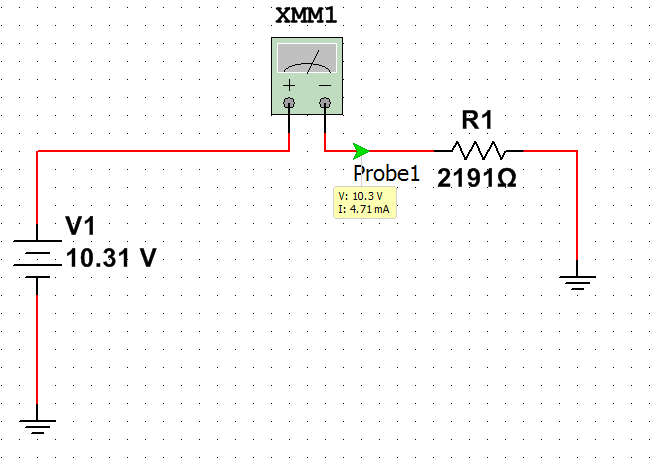
\includegraphics[width=4in]{Circuit_1.PNG} 
   \caption{Circuit 1 (Multisim)}
   \label{fig:example}
\end{figure}

\newpage

\begin{figure}[h!] %  figure placement: here, top, bottom, or page
   \centering
   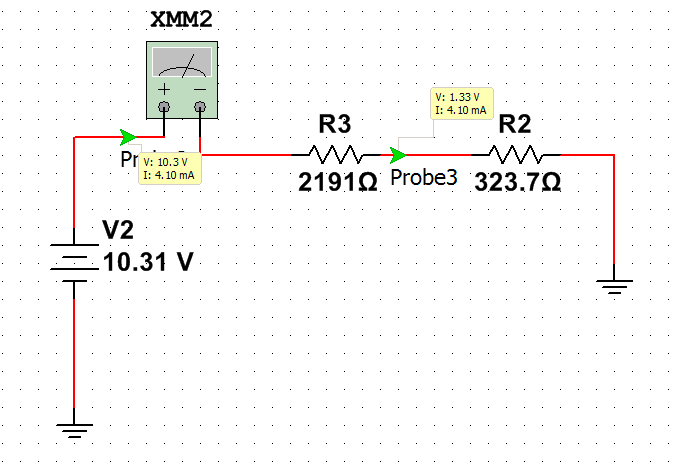
\includegraphics[width=4in]{Circuit_2.PNG} 
   \caption{Circuit 2 (Multisim)}
   \label{fig:example}
\end{figure}

\begin{figure}[h!] %  figure placement: here, top, bottom, or page
   \centering
   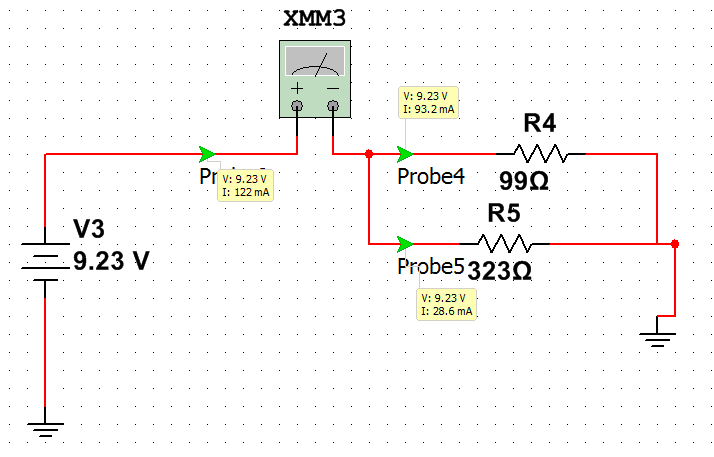
\includegraphics[width=4in]{Circuit_3.PNG} 
   \caption{Circuit 3 (Multisim)}
   \label{fig:example}
\end{figure}

\newpage

\begin{figure}[h!] %  figure placement: here, top, bottom, or page
   \centering
   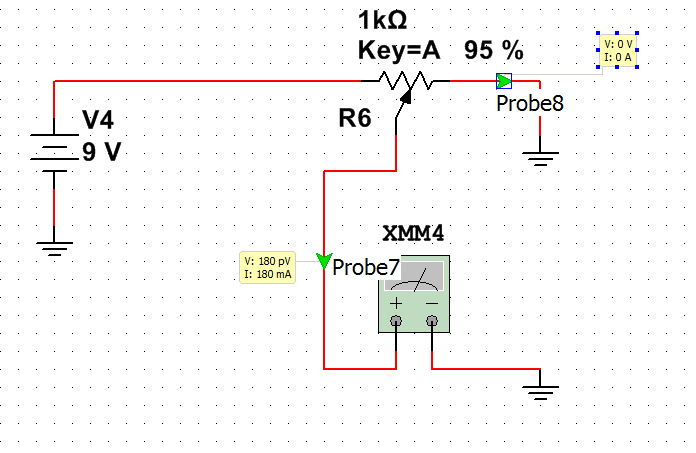
\includegraphics[width=4in]{Circuit_4.PNG} 
   \caption{Circuit 4 (Multisim)}
   \label{fig:example}
\end{figure}


\begin{figure}[h!] %  figure placement: here, top, bottom, or page
   \centering
   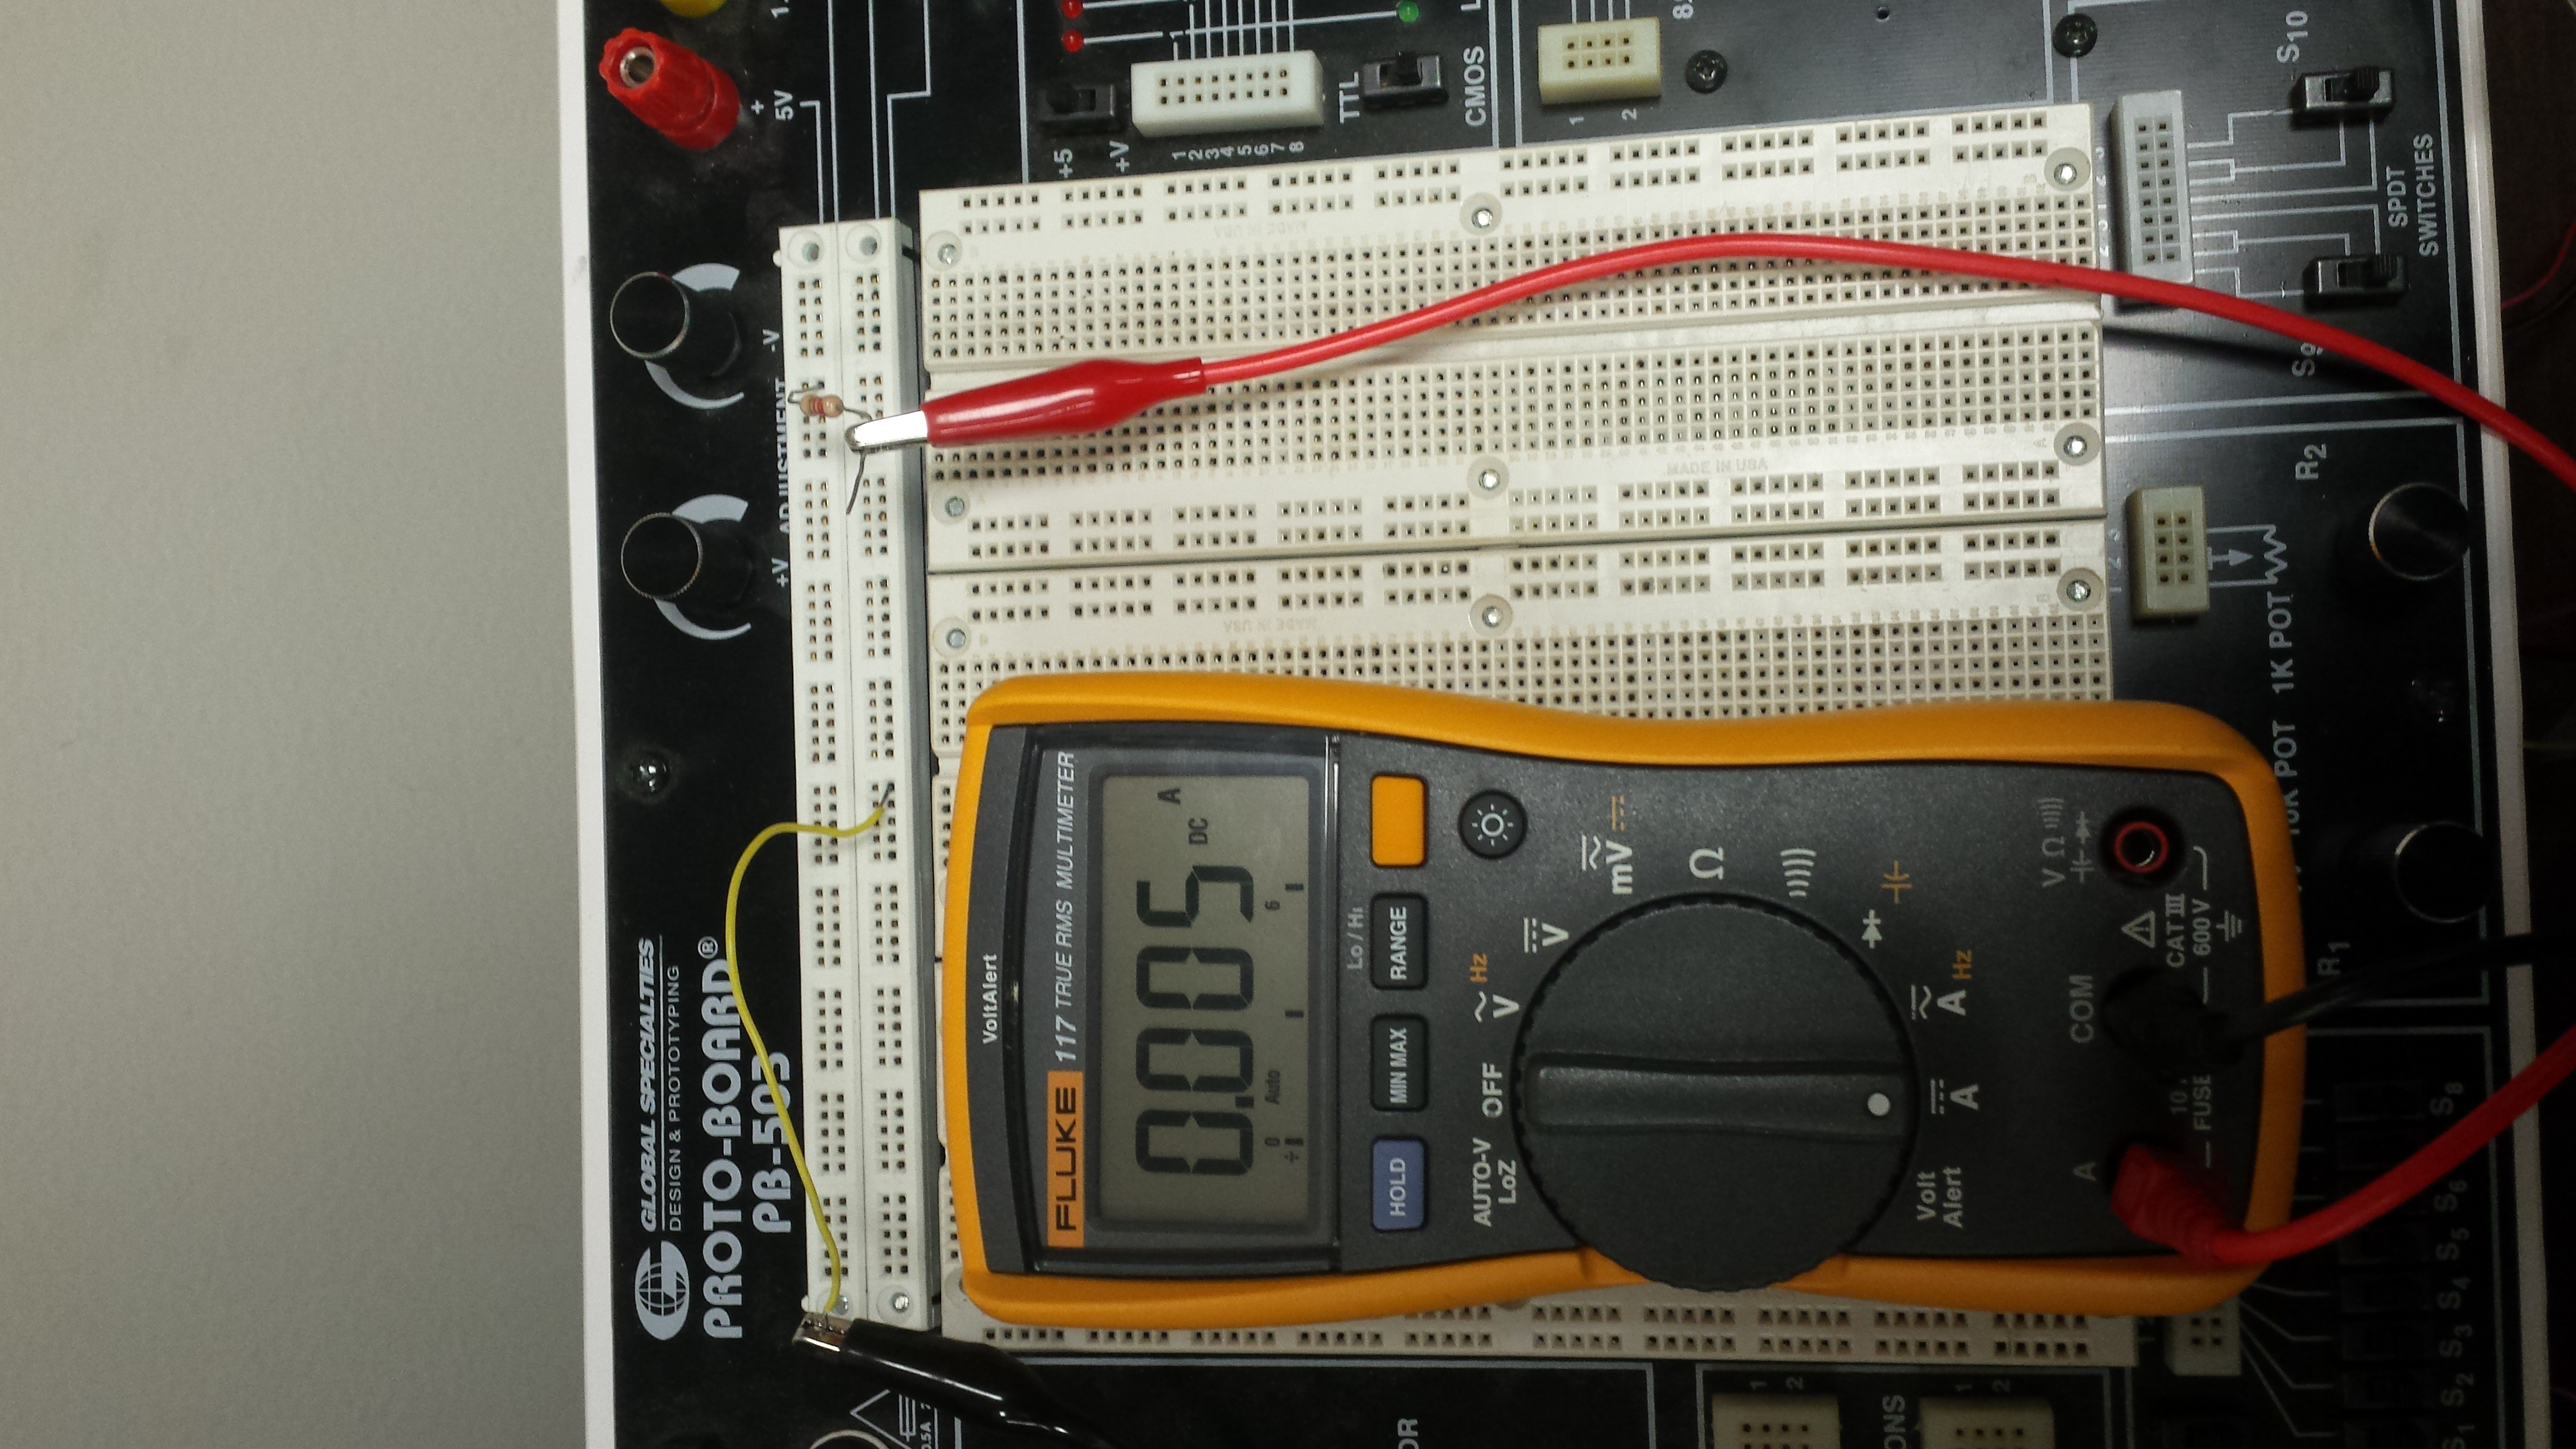
\includegraphics[width=4in,angle=-90]{Circuit_1_real.jpg} 
   \caption{Circuit 1 (Physical)}
   \label{fig:example}
\end{figure}

\newpage

\begin{figure}[h!] %  figure placement: here, top, bottom, or page
   \centering
   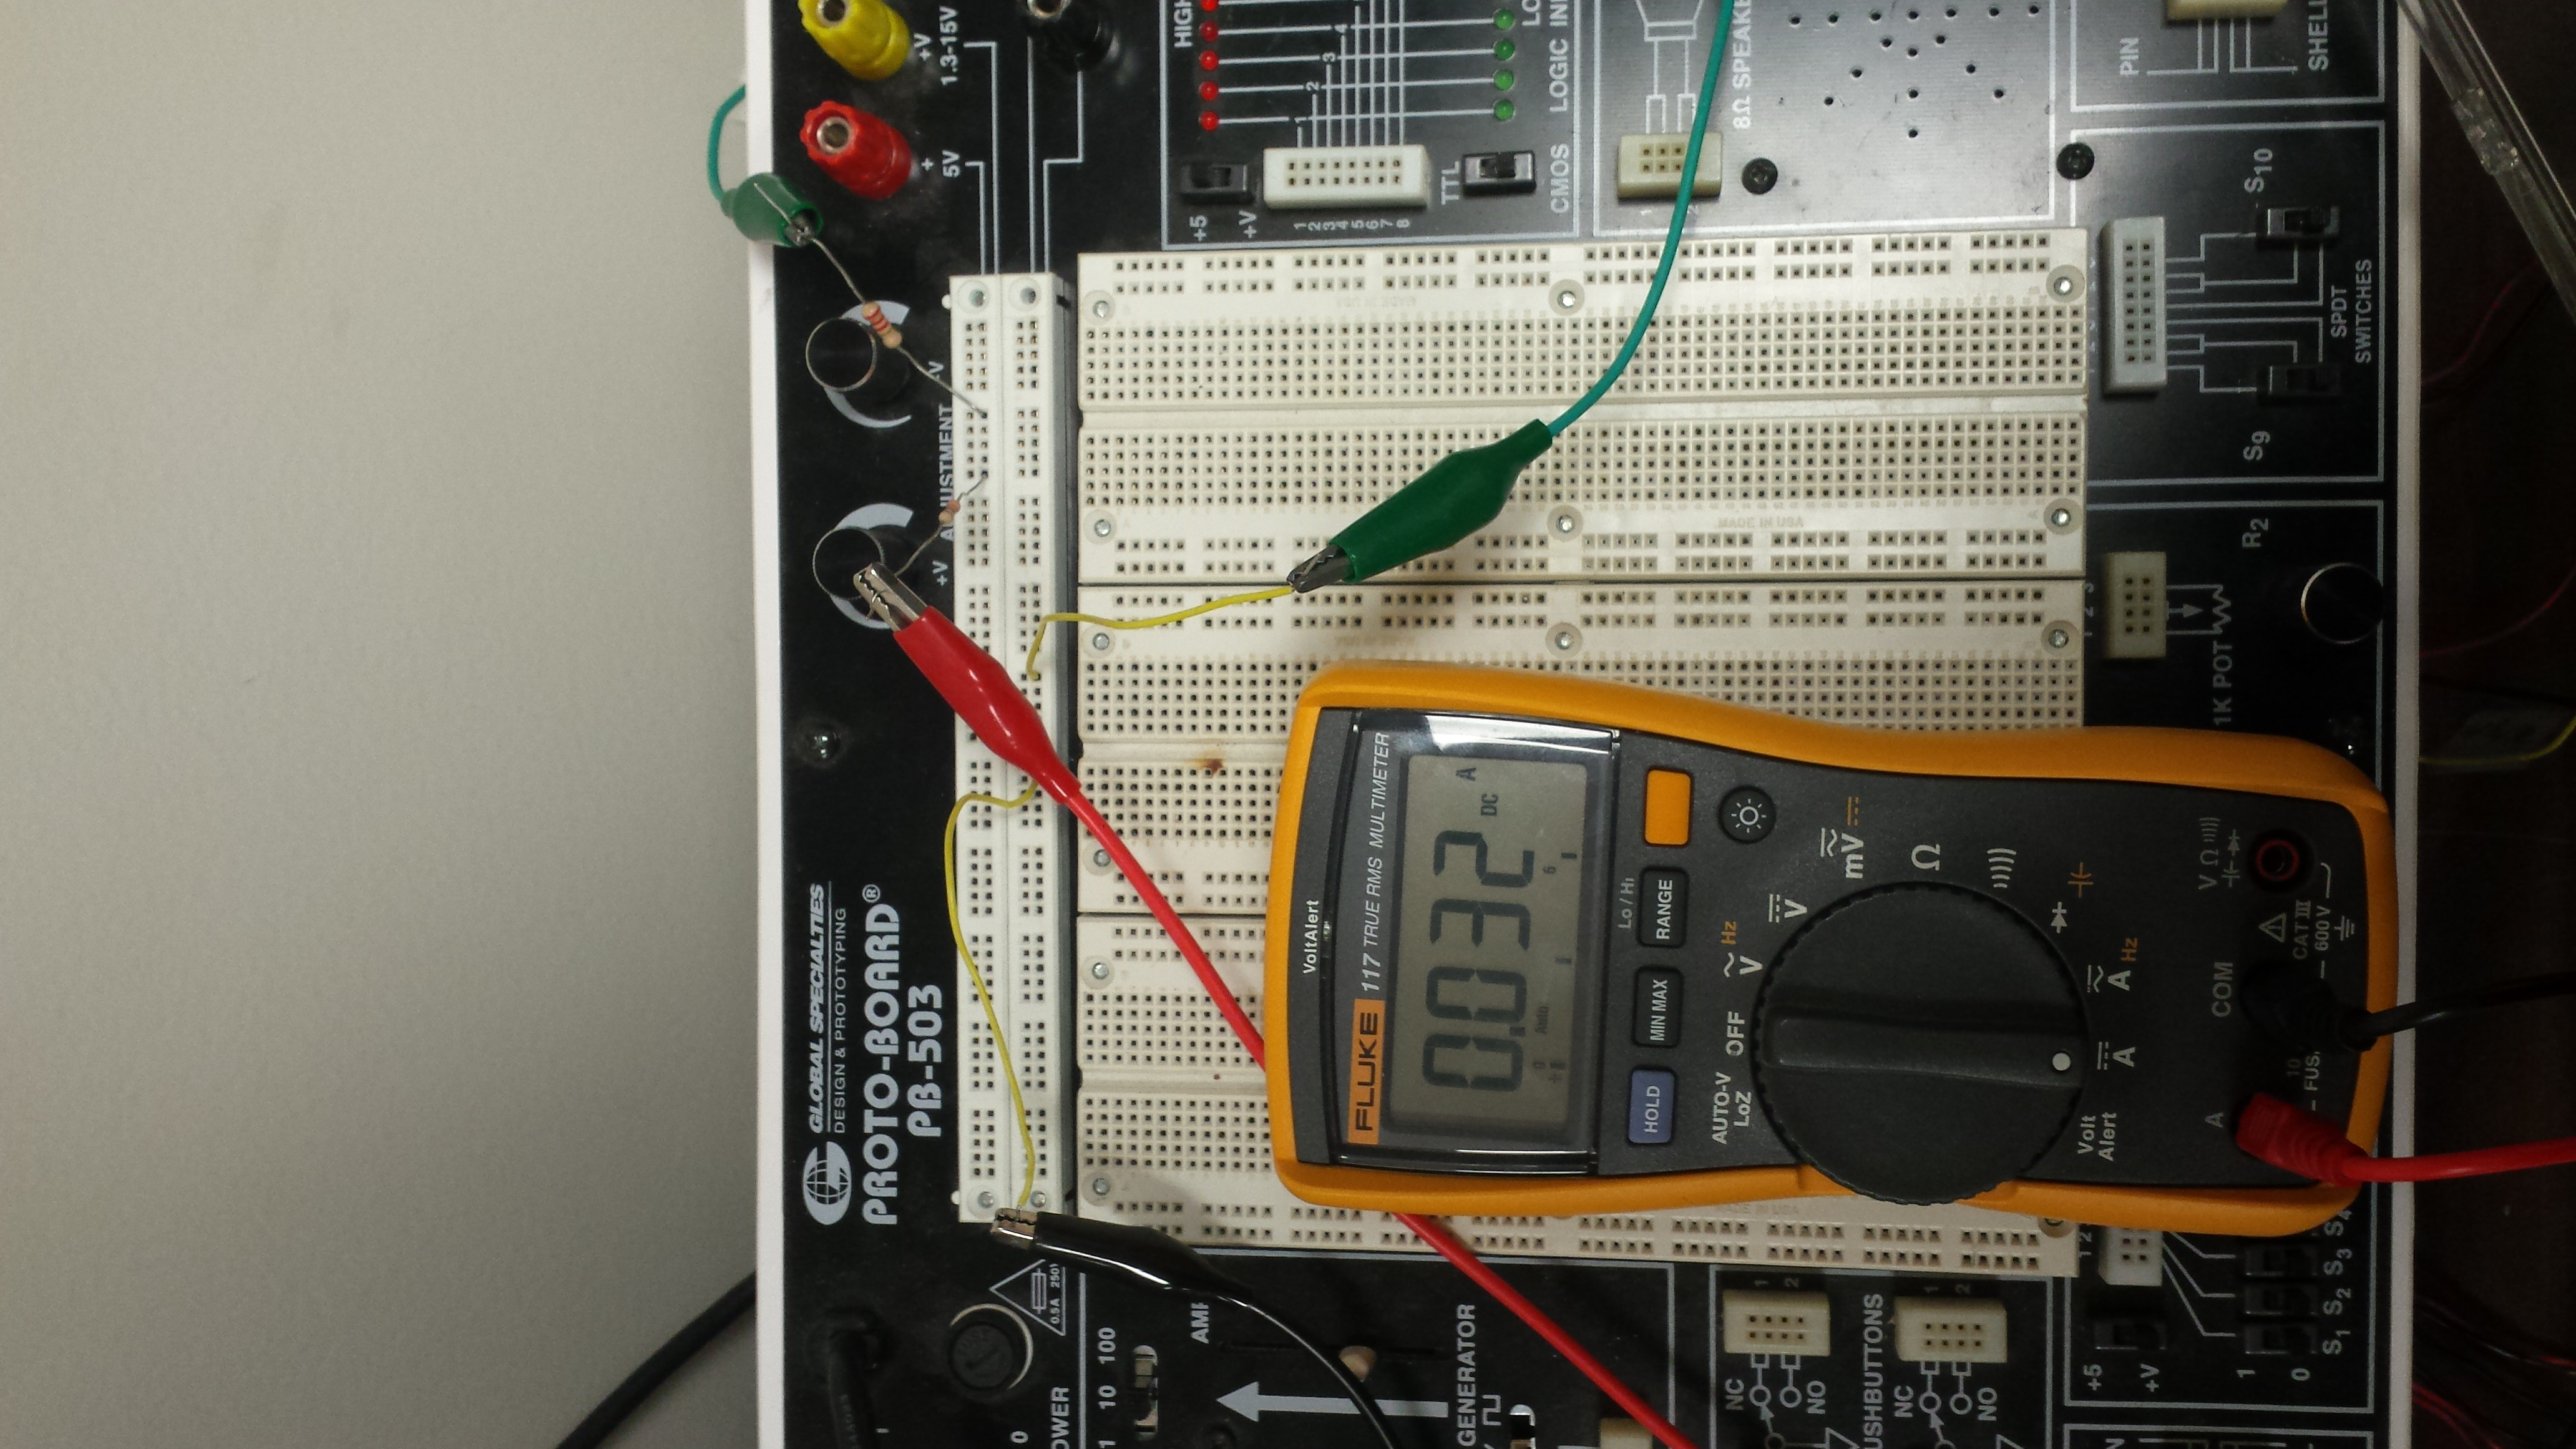
\includegraphics[width=3.5in,angle=-90]{Circuit_2_real.jpg} 
   \caption{Circuit 2 (Physical)}
   \label{fig:example}
\end{figure}

\begin{figure}[h!] %  figure placement: here, top, bottom, or page
   \centering
   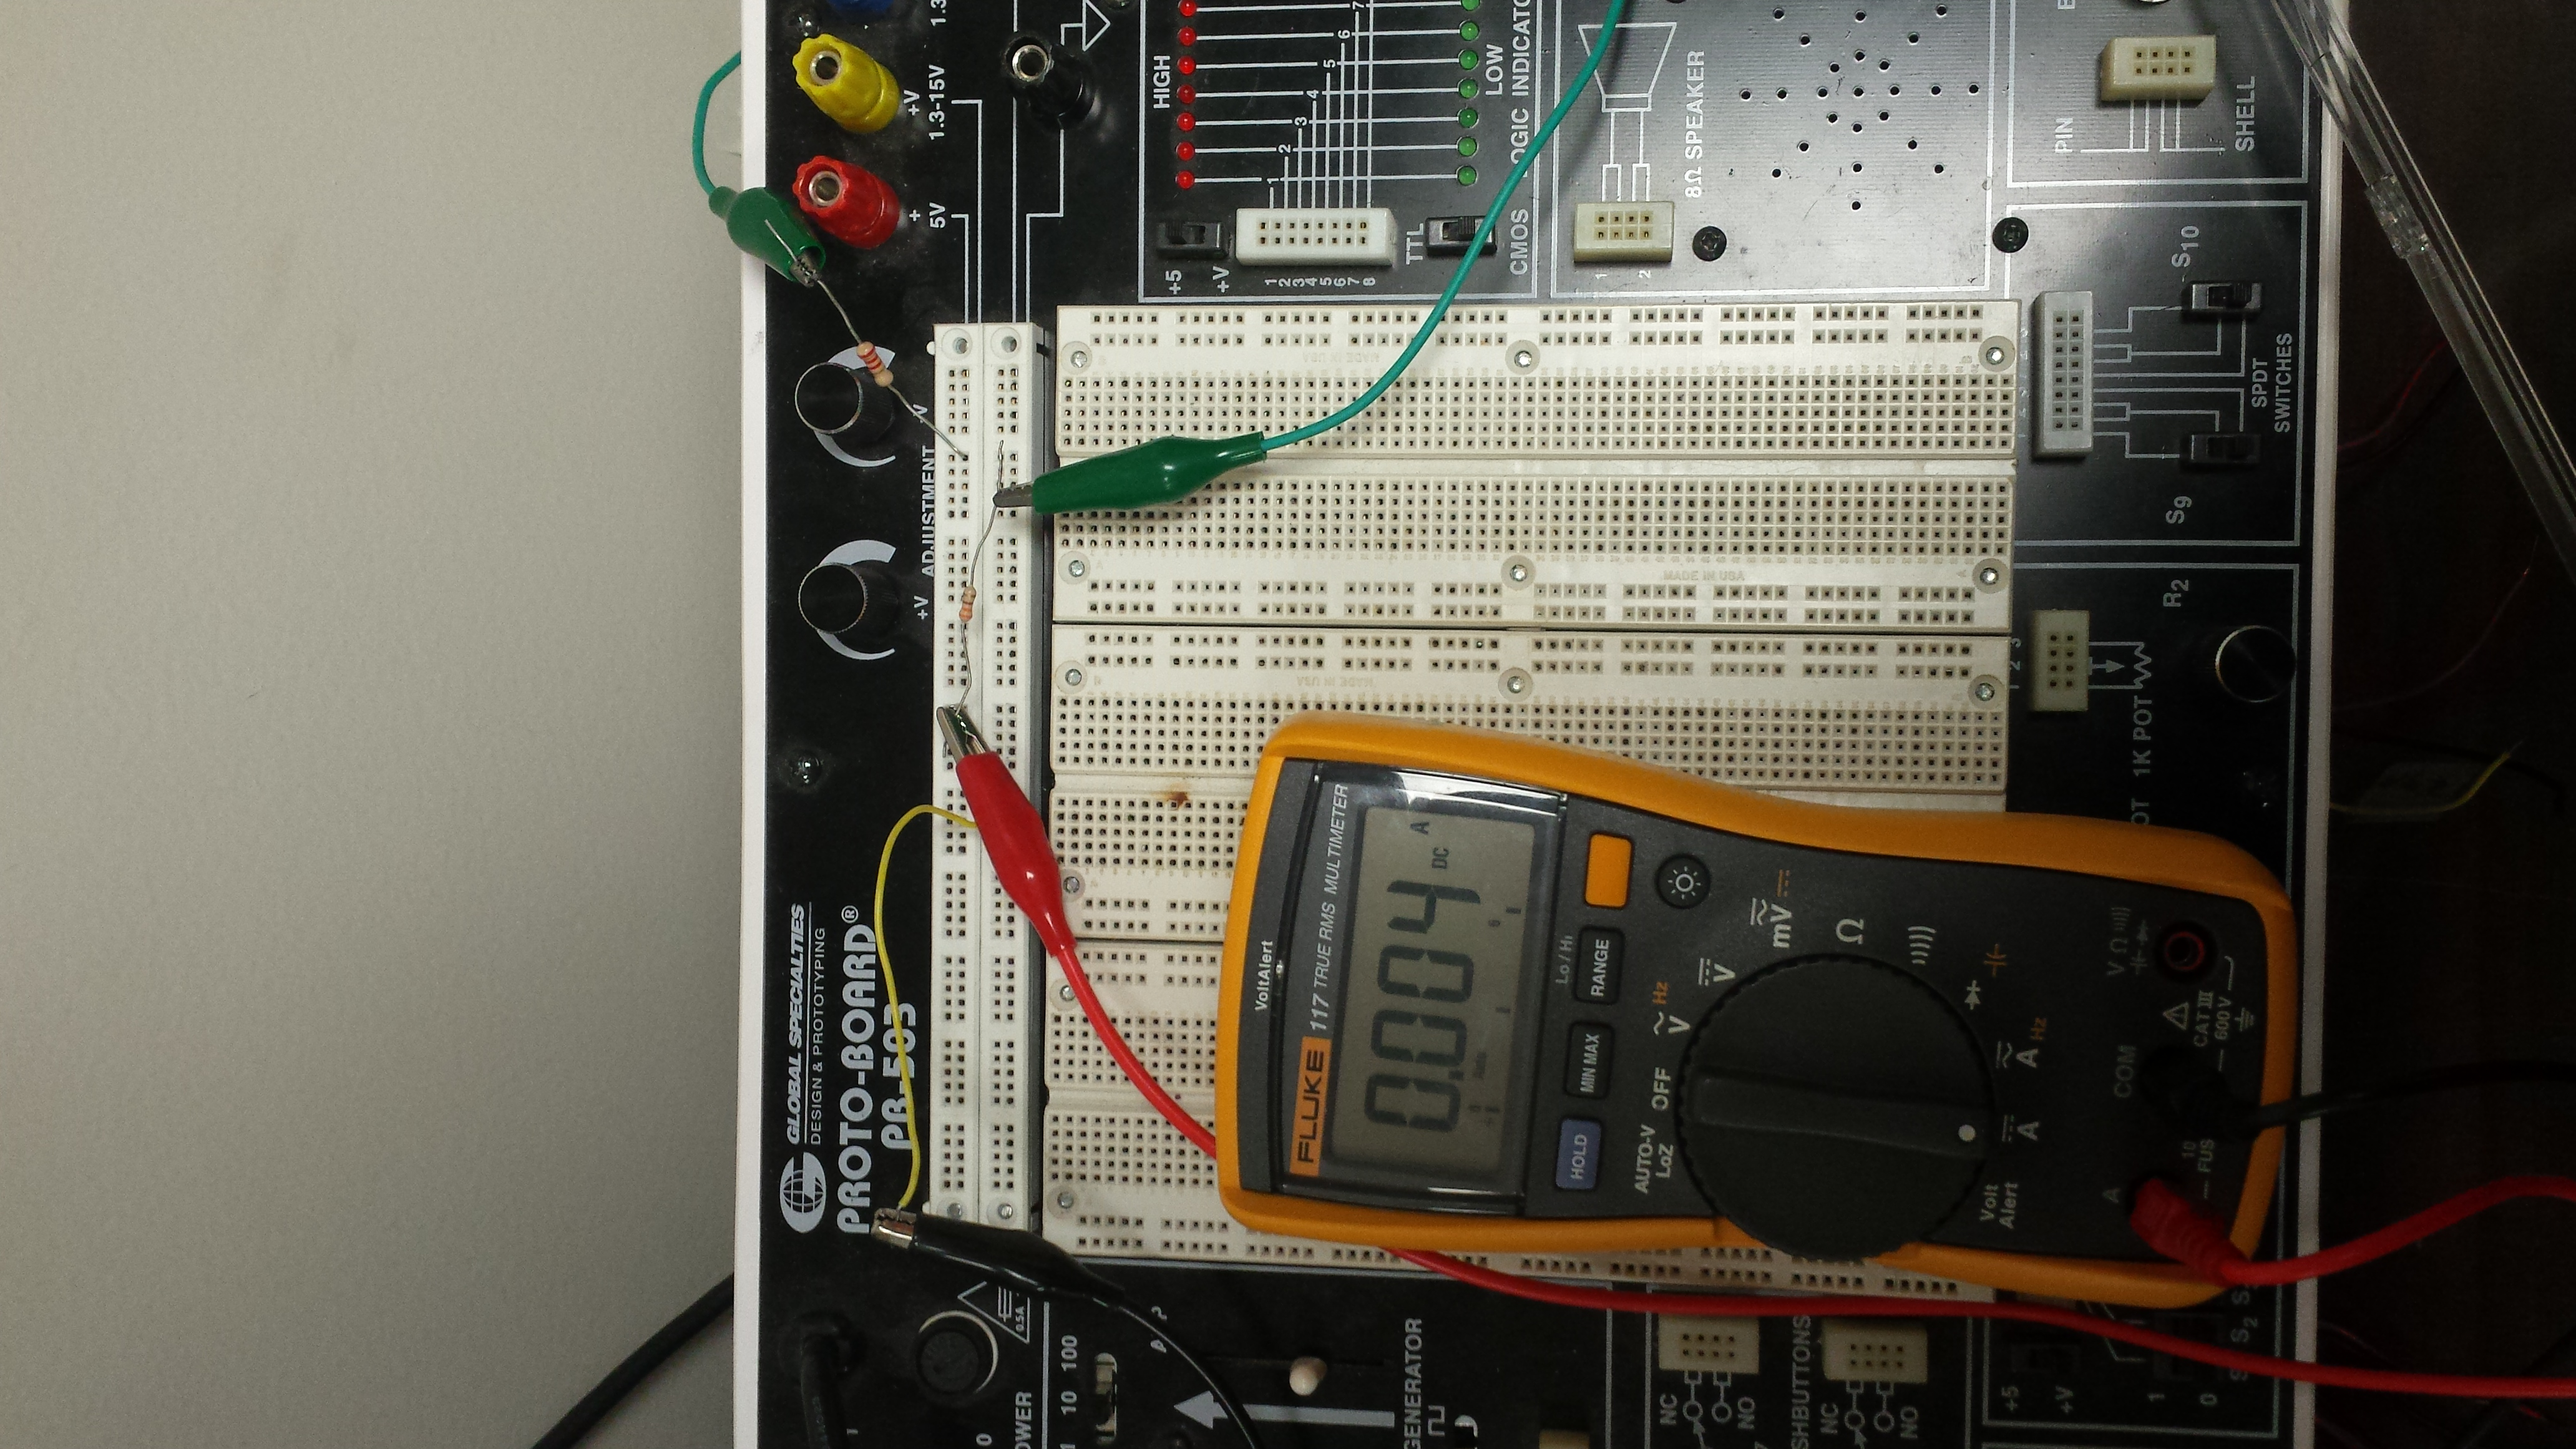
\includegraphics[width=3.5in,angle=-90]{Circuit_3_real.jpg} 
   \caption{Circuit 3 (Physical)}
   \label{fig:example}
\end{figure}

\newpage

\begin{figure}[h!] %  figure placement: here, top, bottom, or page
   \centering
   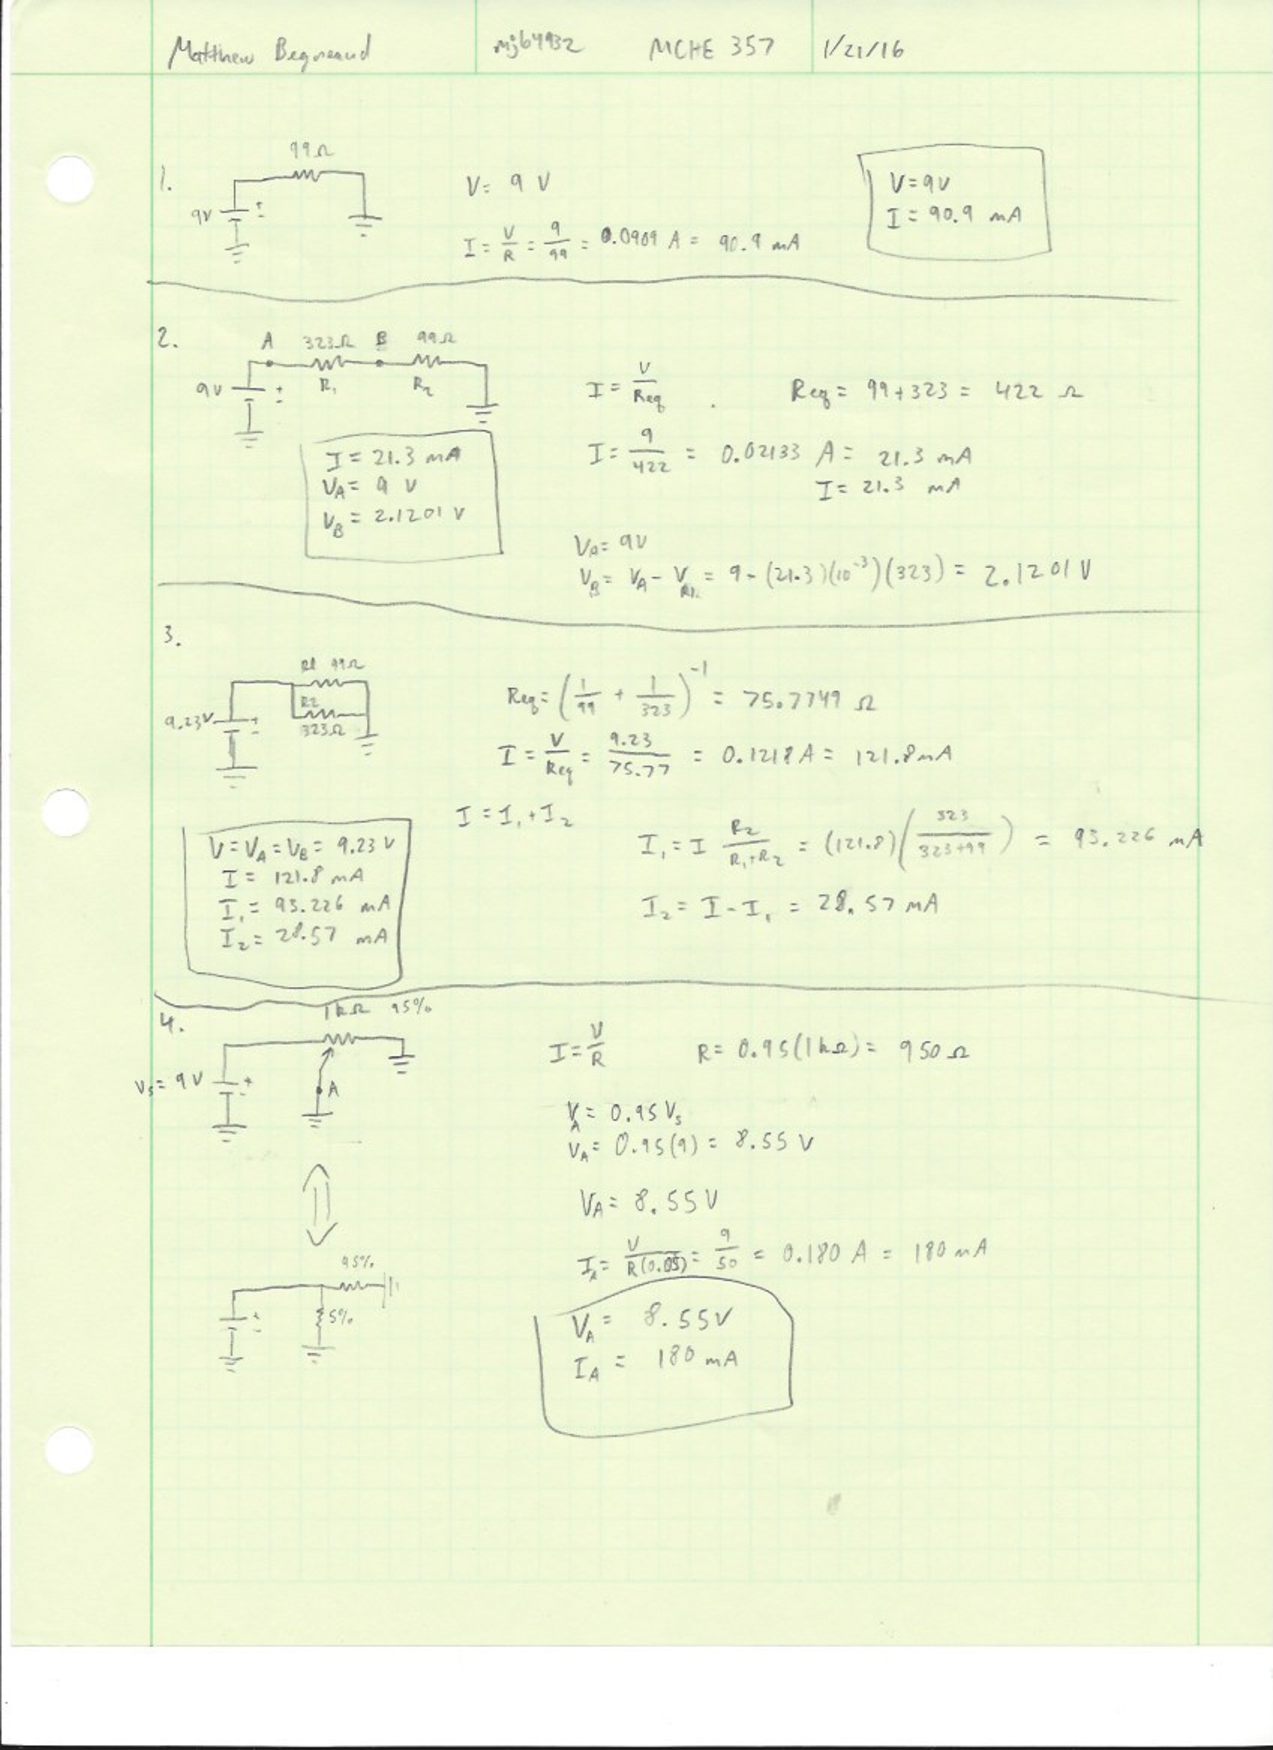
\includegraphics[width=6in]{Multisim_calculations.pdf} 
   \caption{Multisim Calculations}
   \label{fig:example}
\end{figure}

\newpage

\begin{figure}[h!] %  figure placement: here, top, bottom, or page
   \centering
   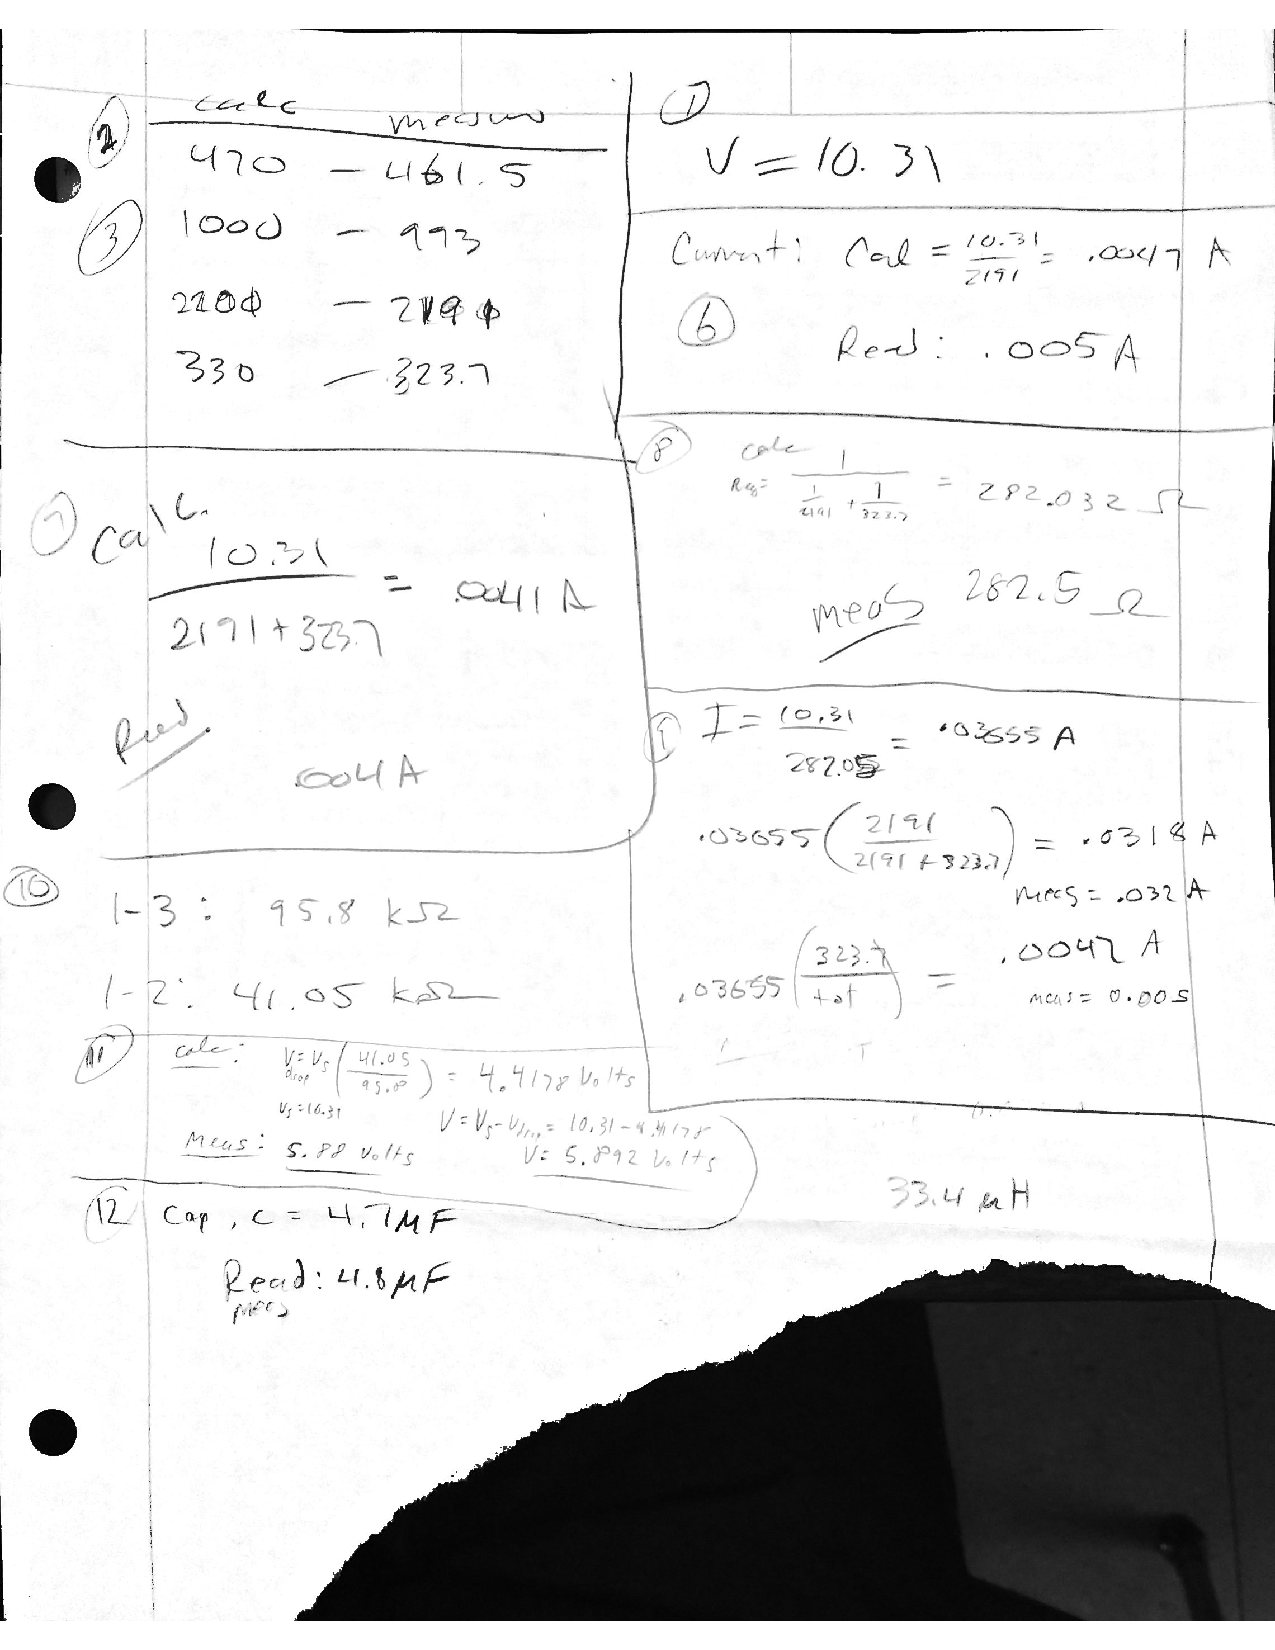
\includegraphics[width=6in]{calculations_real.pdf} 
   \caption{Physical Circuit Calculations}
   \label{fig:example}
\end{figure}

\newpage

\section*{\fontsize{12}{12}\selectfont \large Conclusion}
\addcontentsline{toc}{section}{Conclusion} % Add for each section
This lab demonstrated the principles of basic electrical components. These devices include resistances, capacitors, and inductances. Equivalent resistances was also studied heavily in this lab. Ohm's Law and Kirchhoff's Laws were also studied and used in this lab. The principles learned about basic circuits in this lab will serve as a foundation for understanding future labs.




%\section*{\fontsize{12}{12}\selectfont \large References}

\begin{thebibliography}{2}

% Example
%\bibitem{Wagner}
%Ng, K., Wagner, S.W., Camelio, J., Emblom, W.J. (2010). ?Experimental Analysis of Micro Tube
%Hydroforming Process.? Transactions of NAMRC of SME, 38, 577-584.

\end{thebibliography}



%\section*{\fontsize{12}{12}\selectfont APPENDIX}

%\begin{table}[h!]
%  \caption{}
%  \includegraphics[width=\linewidth]{table1.png}
%\end{table}




\end{document}







----------------------------Templates-------------------------------

-------------------------Figure-----------------------

\begin{figure}[h!]  
  \centering
    \includegraphics[width=\linewidth]{**file**}
    \caption{Docking Station}
\end{figure}

---------------------------Table-----------------------
\begin{table}[ht]
\caption{Nonlinear Model Results} % title of Table
\centering % used for centering table
\begin{tabular}{c c c c} % centered columns (4 columns)
\hline\hline %inserts double horizontal lines
Case & Method\#1 & Method\#2 & Method\#3 \\ [0.5ex] % inserts table
%heading
\hline % inserts single horizontal line
1 & 50 & 837 & 970 \\ % inserting body of the table
2 & 47 & 877 & 230 \\
3 & 31 & 25 & 415 \\
4 & 35 & 144 & 2356 \\
5 & 45 & 300 & 556 \\ [1ex] % [1ex] adds vertical space
\hline %inserts single line
\end{tabular}
\label{table:nonlin} % is used to refer this table in the text
\end{table}



probably best to insert as an image from excel

\bigskip\\
\begin{table}[h!]
  \caption{}
  \includegraphics[width=\linewidth]{**file**}
\end{table}
\bigskip\\





-----------------------------Equations------------------------
-----------------------------Regular
\begin{equation}
a = b + c
\end{equation}

--------------------------------- Multiline
\begin{multline}
a = b + c + d + e + f
+ g + h + i + j \\
+ k + l + m + n + o
\end{multline}

-------------------------------Citations-------------------------
\bibitem{Author last name}
  Last, First., year of publication,
  article name, book(etc) name, from \\
  link goes here

----------------------------------other-----------------------------

equations:
http://moser-isi.ethz.ch/docs/typeset_equations.pdf

citations:
http://library.missouri.edu/engineering/about/guides/asme
https://www.asme.org/shop/proceedings/conference-publications/references